\subsection*{Модель Тобина}
\addcontentsline{toc}{subsection}{Модель Тобина}

\textbf{Задание:}\\
Провести численный анализ и качественный анализ модели Тобина в среде AnyLogic.\\

\textbf{Решение:}\\
Рассмотрим модель монетарных циклов Тобина. Предполагается, что благосостояние населения может обеспечиваться несколькими взаимоисключающими путями. Деньги, бесплатно генерируемые (вводимые в оборот) правительством, служат мерой. Деньги требуются для проведения сделок и инвестиции. Спрос на деньги зависит от распределения доходов и благосостояния населения. Однако для простоты мы предположим, что денежный спрос на душу населения является функцией дохода на душу населения, благосостояния на душу населения и прибыли, ожидаемой при данном вложении капитала. Предполагается, что денежный рынок всегда находится в равновесии, т. е. спрос на деньги всегда равен предложению.\\

$s = (1 - c)$ -- предельная склонность к сбережению\\
$k$ -- капитал\\
$x$ -- количество денег в реальных ценах на душу населения\\
$n$ -- фиксированная скорость роста населения\\
$z$ -- постоянная скорость роста номинальных денежных накоплений\\
$q$ -- динамика скорости изменения цен\\
$g$ -- функция взаимодействия капитала и цен

\begin{align*}
	\begin{cases}
		\dfrac{dk}{dt} = s f(k) - (1 - s)(z - q)x - nk\\[10pt]
		\dfrac{dx}{dt} = x(z - \alpha[x - g(k, q)] - n)\\[10pt]
		\dfrac{dq}{dt} = \beta (\alpha [x - g(k, q)] - q)
	\end{cases}
\end{align*}

\newpage

Решив систему уравнений, получим точку, тип состояний равновесия которой -- седло. (Рисунок \ref{fig:tobin1})
\begin{figure}[h]
	\centering 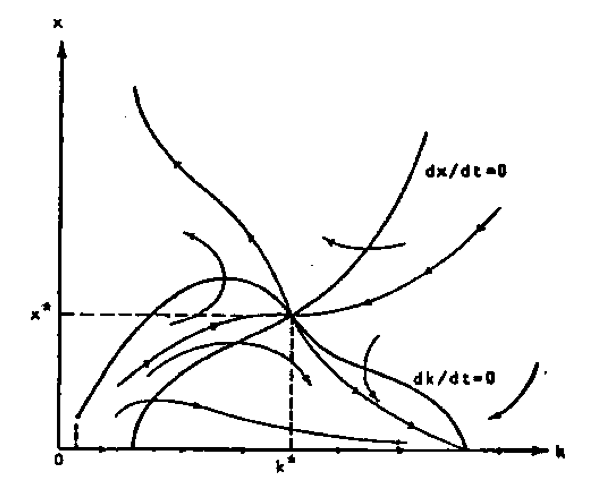
\includegraphics[scale=1]{tobin1}
	\caption{Состояние равновесия модели Тобина}
	\label{fig:tobin1}
\end{figure}

Рассмотрим процессы, происходящие в точке равновесия при возрастании объема денежной массы. Немедленным следствием этого является повышение уровня цен, и реальный объем денежных запасов стремится вернуться к прежнему уровню, однако первоначальное возрастание денежной массы приводит к повышению ценовых ожиданий и снижает наколенный капитал. Оба эти эффекта вызывают падение денежного предложения и могут стать причиной того, что объем денежных запасов будет превышать свое равновесное значение. Если денежное предложение продолжает падать ниже уровня равновесия, переменные меняются местами: объем накопленного капитала возрастает, а ожидания снижаются. В сочетании с прямым влиянием объема денежных запасов на денежные накопления это приведет к изменению направления динамики денежных запасов. Т.о. возникают долговременные колебания. Доказать существование предельного цикла можно используя теорему Хопфа, или построив фазовый портрет на основе численного анализа.

\newpage

В соответствии с формулами, данная модель была реализована в среде моделирования AnyLogic. (Рисунок \ref{fig:tobin2})
\begin{figure}[h]
	\centering 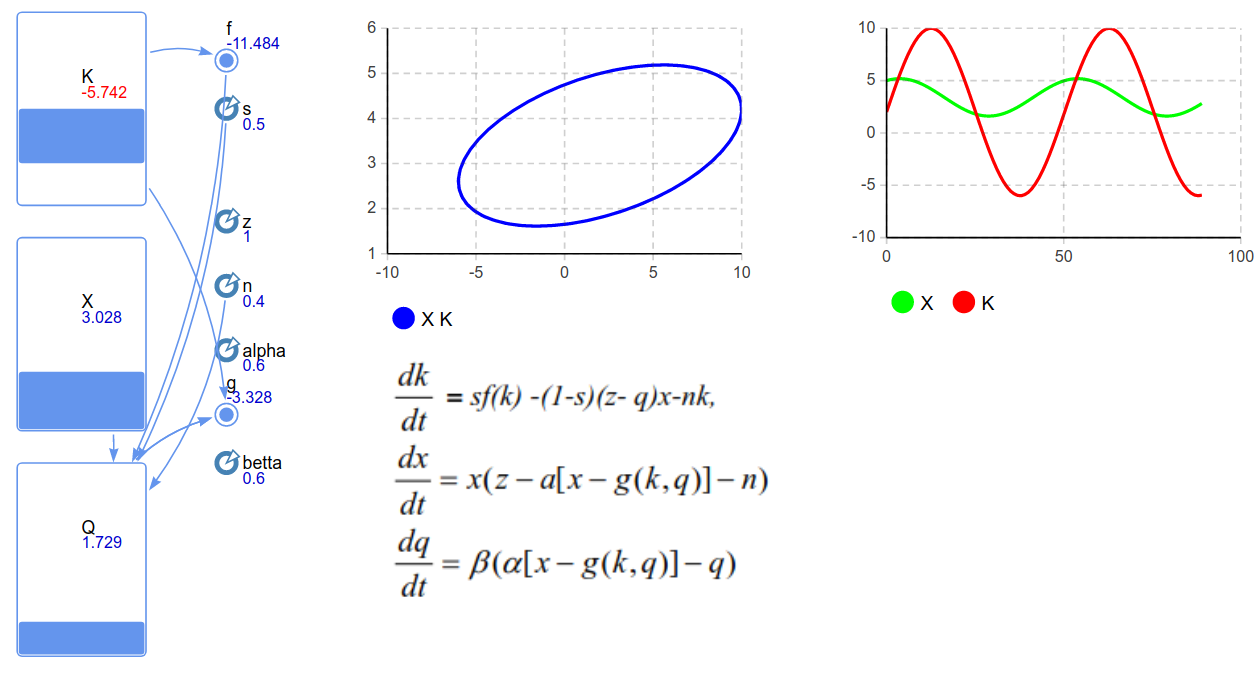
\includegraphics[scale=0.3]{tobin2}
	\caption{Результаты построения модели Тобина в AnyLogic}
	\label{fig:tobin2}
\end{figure}

Таким образом, был проведён численный и качественный анализ модели Тобина.\\